\section{Spécifications}

\subsection{Définition}
Un \texttt{Signal[T]} représente une information de type \texttt{T} dont la disponibilité ou la valeur peut varier avec le temps. À tout moment, il peut se trouver dans l'un des deux états suivants:
\begin{enumerate}
	\item \texttt{Undefined}: le signal ne possède pas de valeur définie,
	\item \texttt{Defined(value)}: le signal possède actuellement la valeur \texttt{value}
\end{enumerate}

Il peut être vu comme une extension de \texttt{Future[T]}. De façon similaire, il représente la présence ou l'absence d'information au fil du temps, mais à la différence de \texttt{Future}, il est autorisé à changer d'état un nombre arbitraire de fois tandis que l'état d'un \texttt{Future} est figé une fois celui-ci résolu.

Le type \texttt{Signal[T]} est covariant avec son paramètre \texttt{T}. L'interface exposée ne permettant que l'accès à la valeur du signal ou sa transformation par le biais de la construction d'un nouveau signal, une instance \texttt{Signal[B]} est substituable à \texttt{Signal[A]} si \texttt{B <: A}\footnote{\texttt{B <: A} désigne une relation de sous-type (\texttt{B extends A})}.

L'état d'un signal peut être dépendant de l'état d'un ou plusieurs autres signaux. Il constitue alors un signal \emph{enfant} associé à un ensemble de signaux \emph{parents}. Cet ensemble peut varier dynamiquement au fil du temps. Un signal enfant ne peut changer d'état que lorsque au moins l'un des ses signaux parents change d'état.

À l'inverse, un signal qui ne dépend d'aucun autre est appelé une \emph{source}. Le changement d'état d'un signal source ne peut s'opérer que par une mutation explicite, extérieur au système de signaux.

\texttt{Signal} vérifie les trois axiomes des monades \cite{haskell-monad-laws}:
\begin{align*}
Signal(x) \text{ flatMap } f &\equiv f(x) \\
a \text{ flatMap } (x \mapsto Signal(x)) &\equiv a \\
(a \text{ flatMap } f)  \text{ flatMap } g &\equiv
a \text{ flatMap } (x \mapsto f(x)  \text{ flatMap } g) 
\end{align*}
Ici, l'opérateur $\equiv$ désigne une équivalence structurelle: les deux expressions sont substituables sans affecter le comportement du programme.

\subsection{Accès à l'état courant}
L'interface d'un signal \texttt{Signal[T]} défini deux méthodes pour accéder à sa valeur courante:
\begin{enumerate}
	\item \textbf{\texttt{Signal.option}}: retourne la valeur courante d'un signal sous la forme d'une \texttt{Option[T]}. C'est une façon sûre d'accéder à l'état du signal quel qu'il soit.
	
	\item \textbf{\texttt{Signal.value}}: retourne la valeur courante du signal (donc une valeur de type \texttt{T}) s'il est défini ou lance une exception\footnote{De type \texttt{UndefinedSignalException}} s'il ne l'est pas. De façon générale, cette méthode est plutôt destinée à être utilisée dans le cadre de la définition de signaux expression (section \ref{sec:sig-expr}) puisque dans ce cas, l'exception est traitée par le constructeur et entraîne la construction d'un signal vide.
\end{enumerate}

Dans le cas où il est nécessaire d'être informé des futurs changements d'états du signal, le mécanisme d'observateur (§~\ref{sec:sig-obs}) peut être utilisé.

\subsection{Pureté et modes d'évaluation} \label{sec:sig-pureness}
Un signal est considéré comme une construction fonctionnelle semi-pure: il n'est dépendant d'aucun état global à l'exception d'autres signaux et ne présente pas d'effets de bords. Ces contraintes s'étendent également aux fonctions utilisées dans leur définition ou transformation par le biais de méthodes telles que \texttt{map} ou \texttt{filter}. Le langage Scala ne permettant pas d'imposer la notion de pureté aux fonction, il est de la responsabilité du développeur de s'assurer que cette contrainte soit respectée.

Cette contrainte découle principalement de l'existence de deux modes d'évaluations pour les signaux qui définissent à quel moment l'état d'un signal enfant doit être calculé après le changement d'état d'un de ses signaux parent:

\begin{enumerate}
	\item \emph{Paresseux}: l'état du signal enfant est réévalué à la demande, lorsque son état courant est accédé et après un changement d'état d'au moins un des ses signaux parents,
	\item \emph{Différé}: l'état du signal enfant est réévalué à la fermeture d'un contexte de mutation impliquant la modification d'au moins un signal parent.
\end{enumerate}

Le mode d'évaluation paresseux est le mode utilisé par défaut pour les signaux. Il offre l'avantage de réduire le nombre d'états à calculer dans le cas où un signal n'est pas accédé aussi fréquemment que son état ne change. Il n'offre cependant aucune garantie concernant le moment auquel une fonction utilisée comme définition d'un signal ou d'une transformation sera appelée, ni même qu'elle sera un jour appelée. Il est donc particulièrement important que ces fonctions respectent également la contrainte de pureté des signaux pour ne pas introduire des comportements non-déterministes dans l'application.

Le mode différé n'est utilisé que dans les situations où l'événement de changement d'état est significatif en plus de la valeur de ce nouvel état. C'est par exemple le cas de l'opération \texttt{fold} (§ \ref{sec:sig-op-fold}) qui est utilisée pour combiner les états successifs d'un signal parent afin de construire l'état du signal enfant. Dans une telle situation, l'utilisation du mode paresseux rendrait le signal enfant non-déterministe puisque son état serait dépendant de la fréquence à laquelle il est accédé \footnote{Si la fréquence d'accès est inférieure à la fréquence de changement d'état du signal parent, certains états seront \emph{manqués} par l'opération de combinaison.}.

Par ailleurs, entre les changements d'états d'un signal parent, l'état d'un signal enfant est gardé en mémoire. L'objectif est d'éviter de devoir recalculer l'ensemble d'une hiérarchie de signaux à chaque accès d'un signal enfant. La valeur d'un signal enfant n'étant pas sensé changer sans un changement d'état d'un parent.

En résumé, l'usage combiné de la \emph{memoization} et de l'évaluation paresseuse rend le timing d'évaluation des fonctions utilisées pour la définition et la transformation de signaux imprévisible, d'autant plus lorsque l'application et la structure de graphe de signaux se complexifie. Respecter la contrainte de pureté lors de l'utilisation des signaux permet de s'affranchir de cette complexité et de se concentrer sur la logique métier de l'application développée.

\subsection{Hiérarchie simplifiée}
La figure \ref{fig:sig-simple-hierarchy} présente une version simplifiée de la hiérarchie des signaux. Seules les informations pertinentes à l'utilisation des signaux ont été conservée: les méthodes, interfaces, classes intermédiaires relevant des détails d'implémentation ne sont pas incluses. La hiérarchie complète formée par les signaux est présentée en section \ref{sec:sig-hierarchy}.

\begin{figure}[!h]
	\centering
	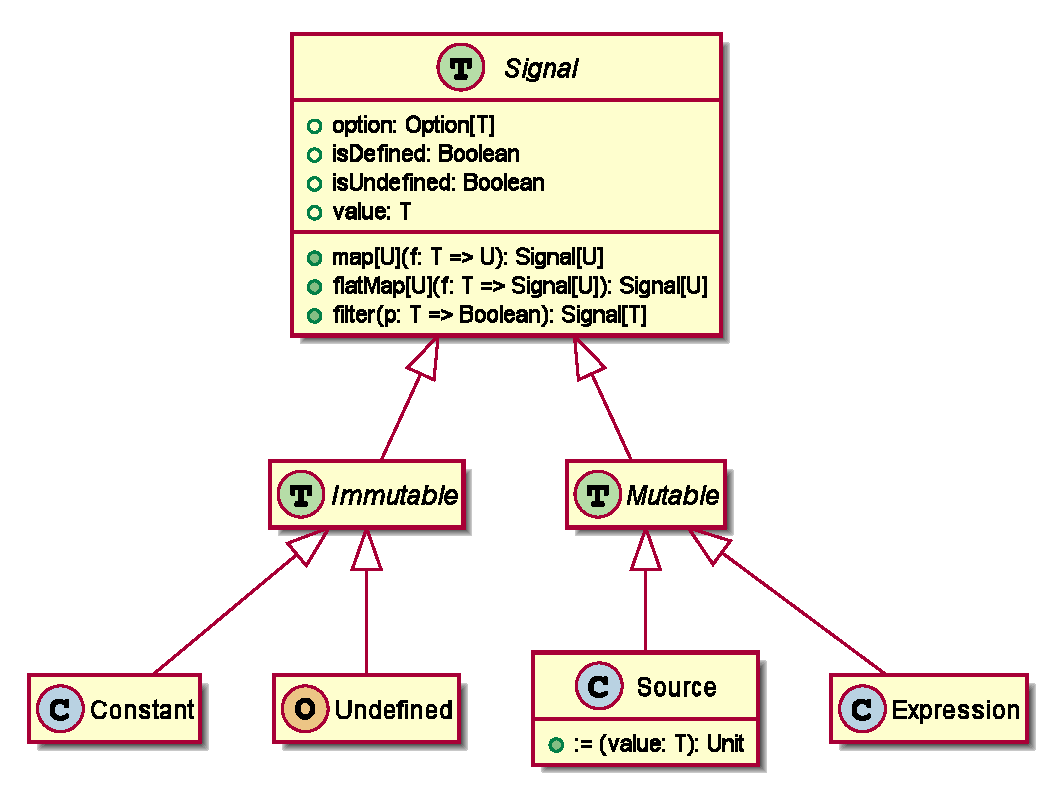
\includegraphics[width=12cm]{img/signals_simple}
	\caption{Hiérarchie simplifiée des signaux}
	\label{fig:sig-simple-hierarchy}	
\end{figure}

Le trait racine \texttt{Signal} est l'interface générique destinée à être manipulée par le développeur, quelque soit le type concret de signal manipulé. Il expose les méthodes nécessaires à l'accès à l'état courant du signal ainsi qu'à la construction de signaux dérivés par transformation. C'est une interface immutable qui ne permet de modifier l'état courant du signal.

La séparation des signaux en deux sous-arbres --- \texttt{Mutable} et \texttt{Immutable} --- capture les différences sémantiques liées à la présence ou l'absence d'une garantie d'immutabilité de l'état d'un signal.

L'intérêt d'un signal dont la valeur ne varie pas peut sembler limité à priori mais se présente lorsqu'une valeur non-signal doit être encapsulée dans un signal afin de satisfaire le système de types. Un tel signal n'a pas de raison de changer d'état au fil du temps, il est alors effectivement immutable. La présence de cette contrainte de façon explicite au niveau de la hiérarchie permet la mise en place d'un certain nombre d'optimisations.

Une instance de la classe \texttt{Constant[T]} est simplement une valeur de type \texttt{T} avec une interface de signal. Un tel signal est toujours dans l'état \emph{défini}.

L'objet singleton \texttt{Undefined} représente quant à lui le signal dont l'état est toujours \emph{indéfini}. Il est généralement référencé à partir de l'objet compagnon du trait \texttt{Signal}: sous la forme \texttt{Signal.undefined}. Puisqu'il n'est jamais défini, il est défini comme une instance de \texttt{Signal[Nothing]}, il est donc par covariance substituable à n'importe quel type de signal \texttt{Signal[T]} \footnote{\texttt{Nothing} est le \emph{bottom type} du système de types en Scala, il est sous-type de tous les types ($\forall \texttt{T}, \texttt{Nothing <: T}$) mais il n'en existe aucune instance.}.

Un signal immutable ne peut être ni \emph{enfant} ni \emph{parent} d'autres signaux. Comme ils ne changent jamais, il n'y a pas de sens de maintenir de graphe de dépendances entre eux. Il n'y aura en effet jamais de propagation de changement d'état à effectuer.

Les opérations de transformation --- \texttt{map}, \texttt{flatMap}, \texttt{filter}, etc. --- appliquées à des signaux constants sont évaluées immédiatement et produisent un nouveau signal constant. Par exemple:

\begin{lstlisting}
val a: Constant[Int] = Constant(2)
val b: Constant[Int] = a.map(_ * 2) // effectuée immédiatement
\end{lstlisting}

\begin{figure}
	\begin{lstlisting}
var i: Int = 0
def f(v: Int): Int = { i += 1; v * 2 }

// Immutable
val a: Constant[Int] = Constant(2)
val b: Constant[Int] = a.map(f)
assert(i == 1) // `f` est évaluée immédiatement

// Mutable
val c: Signal[Int] = Signal(2)
val d: Signal[Int] = c.map(f)
assert(i == 1) // `f` est évaluée de façon paresseuse
assert(d.value == 4) // accès à l'état de `d`, évaluation
assert(i == 2)

// Une sémantique peut en cacher une autre...
val e: Signal[Int] = Constant(2) // typé `Signal`
val f: Signal[Int] = c.map(f)
assert(i == 3)
	\end{lstlisting}
	\caption{Exemple d'évaluation immédiate des transformations}
	\label{fig:constant-eager-transform}
\end{figure}

La figure \ref{fig:constant-eager-transform} illustre ce comportement de façon plus explicite par l'introduction d'effets de bord dans la fonction de transformation utilisée. Cet exemple souligne également l'importance de la pureté des fonctions utilisées en pratique.

Les deux types de signaux mutables, sources (§ \ref{sec:sig-source}) et expressions (§ \ref{sec:sig-expr}), sont décrits plus en détails dans les sections les concernant.

\subsection{Construction}
Un signal est généralement dérivé par transformation de signaux existants. Cependant, dans le cas où un nouveau signal racine doit être construit, deux approches sont disponibles.

La première méthode est l'utilisation des constructeurs offerts par l'objet \texttt{Signal}:

\begin{itemize}
	\item \code{def Signal.apply[T](expr: => T): Signal[T]}
	\item \code{def Signal.define[T](expr: => Option[T]): Signal[T]}
\end{itemize}

L'expression fournie à \texttt{apply} sera évaluée pour déterminer la valeur du signal produit et les dépendances vers d'autres signaux seront automatiquement identifiées. Si l'expression fait référence à l'état d'au moins un signal parent non-constant, un signal de type \texttt{Expression} (§ \ref{sec:sig-expr}) est retourné. Dans le cas où aucun signal parent n'a été accédé, un signal de type \texttt{Constant} est retourné.

La variante \texttt{define} est similaire mais considère une valeur \texttt{None} comme un signal indéfini tandis qu'une valeur \texttt{Some(v)} est considérée comme un signal défini et de valeur \texttt{v}. 

La secondes approche consiste en l'utilisation explicite d'un signal de type \texttt{Source} (§ \ref{sec:sig-source}). 

\subsection{Signal source} \label{sec:sig-source}

Une \texttt{Source[T]} est l'équivalent réactif d'une variable en programmation non-réactive. C'est un conteneur mutable pour une valeur de type \texttt{T}, pouvant être indéfinie. Deux constructeurs sont disponibles selon l'état initial désiré pour la source:

\begin{itemize}
	\item \code{def Source.apply[T](value: T): Source[T]}
	\item \code{def Source.undefined[T]: Source[T]}
\end{itemize}

Une instance de \texttt{Source[T]} offre une méthode de mutation explicite
\begin{center}
	\code{def := (value: T): Unit}
\end{center}
permettant de mettre à jour la valeur contenue dans la source de façon impérative. Cette opération est un changement d'état de la source et provoquera l'invalidation récursive des tous les signaux en dépendant.

Une source est destinée à être utilisées lors de la construction de système hybrides, combinant code impératif basé sur les effets de bords et code fonctionnel. La source est alors un point d'entrée dans le graphe de dépendances des signaux pour la partie de code impérative.

\textit{À ajouter: une opération utilisant une fonction de mutation à partir de l'état courant:}
\begin{lstlisting}
def ~= (f: T => T): Unit = { this := f(value) }
\end{lstlisting}

\subsection{Signal expression} \label{sec:sig-expr}

Un signal expression est un signal dont la définition est une expression arbitraire. Un tel signal détermine automatiquement ses signaux parents en observant les signaux accédés lors de l'évaluation de l'expression et construit ainsi automatiquement son arbre de dépendances. Si l'un de ces signaux venait à changer, la valeur du signal expression serait recalculée.

Il est construit en passant l'expression de définition au constructeur \texttt{Signal} tel qu'illustré par la figure \ref{fig:signal-expr-init}. La variante \texttt{Signal.define} est similaire à la méthode \texttt{apply}, mais reçoit une expression de type \texttt{Option[T]}. Une évaluation de cette expression produisant la valeur \texttt{None} ou une instance \texttt{Some(v)} conduit respectivement à un état indéfini ou défini du signal.

\begin{figure}[!h]
	\begin{lstlisting}
val a: Signal[Int] = ...
val b: Signal[Int] = ...
val c: Signal[Int] = Signal {
	a.value + b.value
}
	\end{lstlisting}
	\caption{Déclaration d'un signal expression}
	\label{fig:signal-expr-init}
\end{figure}

Les parents d'un signal expression sont dynamiques. À chaque évaluation, la liste des parents est vidée puis reconstruite selon l'évaluation actuelle. De cette façon, les dépendances sont toujours le plus précises possible et les invalidation inutiles sont évitées. Ceci est particulièrement important dans le cas de signaux contenant des branches et donc un ensemble de dépendances dynamiques selon l'état d'autres signaux.

Dans l'exemple de la figure \ref{fig:signal-expr-branches}, le signal construit ne dépend de \texttt{b} que si la valeur du signal \texttt{a} est \texttt{false}. Dans le cas contraire, il est dépendant de \texttt{c}. Dans tous les cas, une dépendance est créée vers le signal \texttt{a}.

\begin{figure}[!h]
	\begin{lstlisting}
Signal {
	if (a.value) b.value else c.value
}
	\end{lstlisting}
	\caption{Définition d'un signal expression avec branches}
	\label{fig:signal-expr-branches}
\end{figure}

Selon la situation, l'usage d'une expression pour définir un signal peut se révéler plus simple que la combinaison de nombreuses opérations de transformations élémentaires pour composer le comportement attendu.

Dans les cas les plus complexes, principalement lors de l'utilisation de structures de contrôles tel que des branches conditionnelles, des opérations de \emph{pattern matching} ou des boucles, une expression permet une définition concise et atomique du signal tandis que pour obtenir un résultat équivalent à l'aide des opérateurs de transformation, une longue chaîne de transformations successives, considérablement plus difficile à comprendre, serait nécessaire.

À l'inverse, dans les cas plus simples, une opération de transformation permet de réutiliser un \emph{pattern} de transformation établi, étant alors à la fois plus concis et mentalement plus simple puisqu'il utilise une sémantique clairement établie et commune.

\subsubsection{Contraintes des expressions}

Les signaux doivent être considérés comme des constructions semi-pure d'un point de vue fonctionnel (§~\ref{sec:sig-pureness}). Il est ainsi important que l'expression utilisée comme définition respecte ce principe en ne provoquant aucun effet de bord et en ne dépendant d'aucune valeur mutable qui ne serait pas un signal. En effet, si une valeur mutable non-signal est référencée par une expression, l'état résultant du signal est alors dépendant de l'instant d'évaluation pour lequel aucune garantie n'est fournie.

Il est aussi important que l'évaluation d'une expression s'effectue de façon synchrone. En effet la liste de dépendances du signal est construite lors de l'évaluation de l'expression. Si un signal parent est accédé de façon asynchrone ou \emph{lazy}, la dépendance ne sera pas identifiée et le signal ne sera pas correctement invalidé en cas de changement d'état de ce signal parent.

Les deux principaux suspects à considérer sont \texttt{Future} et \texttt{Stream}. Le premier pour le délai qu'il introduit dans l'évaluation de sa valeur, le second pour sa sémantique \emph{lazy}.

Il est intéressant de noter que la seule observation du paramètre de type du signal permet d'identifier un potentiel problème. En effet un signal de type \texttt{Signal[Int]} dont la définition impliquerait l'utilisation d'une instance de \texttt{Stream} n'est pas un souci; une fois la valeur finale de type \texttt{Int} produite, l'ensemble des éléments pertinents du flux auront été consommés de façon synchrone. Le principe s'applique de façon similaire à l'opération \texttt{Option.orElse} pour laquelle le paramètre est passé \emph{by name}.

À l'inverse, un signal \texttt{Signal[Stream[Int]]} expose l'instance de \texttt{Stream} utilisée. Dans une telle situation, si le calcul d'un élément du flux requiert l'accès à un autre signal, aucune relation de dépendance ne sera établie. Des types de signaux tels que \texttt{Signal[Stream[A => B]]}, \texttt{Signal[Future[A]]} voir même \texttt{Signal[A => B]} indiquent un risque important ne pas respecter la contrainte de synchronisme.

\subsection{Opérateurs de transformations}
Dans les exemples ci-dessous, les opérations sont supposées appliquées à une instance de type \texttt{Signal[T]}, \texttt{T} faisant ainsi référence au type d'élément contenu dans le signal original. Seules les opérateurs les plus courants et ceux utilisées par le compilateur Scala lors de la compilation d'une compréhension \texttt{for} sont traités ici. La Scaladoc du projet contient une liste exhaustive des opérations disponibles.

\subsubsection{Opérateur de transformation simple (\texttt{map})}

\begin{itemize}
	\item \code{def map[U](f: T=>U): Signal[U]}
\end{itemize}

La fonction \texttt{map} effectue une opération de transformation simple sur la valeur d'un signal en appliquant la fonction \texttt{f} à la valeur courante du signal et retournant un nouveau signal contenant en tout temps le résultat de cette transformation. En d'autre termes, lorsque l'état du signal original change, la fonction \texttt{f} est réévaluée avec la nouvelle valeur du signal parent et le signal enfant est mis à jour.

Si le signal d'origine est indéfini, la fonction \texttt{f} n'est pas appliquée et le signal enfant prend également l'état indéfini.

\begin{figure}[h]
	\begin{lstlisting}
val a: Signal[Int] = Source(4)
val b: Signal[Double] = a.map(Math.sqrt(_)) // b.value -> 2.0
a := 9 // b.value -> 3.0

val c: Signal[_] = Signal.undefined // `c` est indéfini
val d: Signal[_] = c.map(value => ???)
d.option == None // la fonction passée à `map` n'est jamais évaluée
	\end{lstlisting}
	\caption{Exemple d'utilisation de \texttt{map}}
\end{figure}

\subsubsection{Opérateur de sélection (\texttt{flatMap})}

\begin{itemize}
	\item \code{def flatMap[U](f: T=>Signal[U]): Signal[U]}
\end{itemize}

Dans le cas des signaux, \texttt{flatMap} implémente une opération de sélection: étant donné un signal \texttt{a} de type \texttt{Signal[T]} et une transformation sous la forme d'une fonction \texttt{f: T => Signal[U]}, la fonction \texttt{f} est appliquée à la valeur actuelle du signal \texttt{a} afin d'obtenir un second signal \texttt{b} de type \texttt{Signal[U]} et retourne un troisième signal \texttt{c} également de type \texttt{Signal[U]} dont la valeur est en tout temps égale à celle du signal \texttt{b}. La fonction \texttt{f} est réévaluée à chaque changement d'état du signal \texttt{a} afin de définir un nouveau signal de référence \texttt{b}.

Si le signal \texttt{a} est indéfini, la fonction \texttt{f} n'est pas appliquée et le signal \texttt{c} est également considéré indéfini.

La fonction \texttt{flatMap}\footnote{\emph{bind} en Haskell, ou \texttt{>>=}} est la fonction universelle de transformation des monades. Elle est suffisamment générale pour permettre de définir toutes les autres fonctions de transformation comme des cas particuliers de \texttt{flatMap}. Par exemple, la transformation \texttt{a.map(f)} peut également s'écrire  sous la forme \texttt{a.flatMap(value => Constant(f(value))}.

\begin{figure}[h]
	\begin{lstlisting}
val choice: Signal[Int] = ...
def selectSignal(choice: Int): Signal[T] = ...
// L'état de `c` est identique à celui du signal retourné par `selectSignal` pour la valeur courante de `choice`
val c: Signal[T] = choice.flatMap(selectSignal)
	\end{lstlisting}
	\caption{Exemple d'utilisation de \texttt{flatMap}}
\end{figure}

\subsubsection{Opérateur de filtrage (\texttt{filter})}

\begin{itemize}
	\item \code{def filter(p: T=>Boolean): Signal[T]}
\end{itemize}

La fonction \texttt{filter} effectue une opération de filtrage d'un signal en appliquant un prédicat \texttt{p} à la valeur courante du signal et retournant un nouveau signal de même valeur si le prédicat est vérifié, ou un signal indéfini si le prédicat n'est pas vérifié.

\begin{figure}[h]
	\begin{lstlisting}
	val a: Signal[Int] = Source(4)
	val b: Signal[Int] = a.filter(_ % 2 == 0) // b.option -> Some(4)
	a := 5 // b.option -> None, b.value -> UndefinedSignalException
	\end{lstlisting}
	\caption{Exemple d'utilisation de \texttt{filter}}
\end{figure}

\subsubsection{Opérateur de combinaison (\texttt{fold} / \texttt{reduce})} \label{sec:sig-op-fold}

\begin{itemize}
	\item \code{def fold[U](a: U)(f: (U, T)=>U): Signal[U]}
	\item \code{def reduce[U >: T](f: (U, T)=>U): Signal[U]}
\end{itemize}

L'opérateur \texttt{fold} permet l'introduction d'un effet de \emph{mémoire} aux signaux. Il prend en paramètre un \emph{accumulateur initial} \texttt{a} de type \texttt{U} et une fonction de combinaison \texttt{f: (U, T) => U} permettant d'associer la valeur courante du signal à cet état pour produire un \emph{accumulateur courant}, également de type \texttt{U}, qui sera alors la valeur du signal produit par l'opérateur.

Lors d'un changement d'état du signal initial, l'\emph{accumulateur antérieur} est combiné à la nouvelle valeur du signal pour former le nouvel \emph{accumulateur courant}. Si le signal est indéfini la fonction \texttt{f} n'est pas évaluée et l'\emph{accumulateur antérieur} devient l'\emph{accumulateur courant} sans modification. Dans le cas où le signal est initialement indéfini, l'\emph{accumulateur initial} devient l'\emph{accumulateur courant} tel quel.

Le signal retourné par \texttt{fold} est toujours défini.

L'opérateur \texttt{fold} possède la particularité d'être affecté par le mode d'évaluation du signal qu'il produit. En mode paresseux, l'opérateur de combinaison ne serait appliqué que lors de l'accès au signal enfant. Il serait alors possible de \emph{manquer} des changements d'état du signal parent. C'est pourquoi les signaux produits par l'opérateur \texttt{fold} ont toujours un mode d'évaluation strict afin d'obtenir un comportement déterministe et indépendant de la façon dont le signal enfant est utilisé.

À l'inverse de la fonction \texttt{fold} présente sur les collections de la bibliothèque standard Scala qui retourne une unique valeur pour une collection. La fonction \texttt{fold} des signaux retourne également un \texttt{Signal}. Le nom \emph{fold} ne fait ainsi pas référence au passage d'une collection à un élément unique, mais à la combinaison successive des différents \emph{états} du signal parent.

\begin{figure}[h]
	\begin{lstlisting}
val a: Signal[Int] = ...
val s: Signal[Int] = a.fold(0)(_ + _)
// Le signal `s` représente la somme de toutes les valeurs du signal `a`.

val b: Signal[Int] = ...
val m: Signal[Int] = b.fold(0)(_ max _)
// Le signal `m` représente la valeur maximale obtenue par le signal `b`.
	\end{lstlisting}
	\caption{Exemple d'utilisation de \texttt{fold}}
\end{figure}

L'opérateur \texttt{reduce} est une variation de l'opérateur \texttt{fold} dont l'\emph{accumulateur initial} est déterminé implicitement par l'état courant du signal parent. À l'inverse de la transformation \texttt{fold}, si l'état courant du signal parent est indéfini, alors le signal enfant est également indéfini. Dès lors que l'état du signal parent sera défini pour la première fois, l'état du signal enfant ne pourra plus être indéfini.

\begin{figure}[h]
	\begin{lstlisting}
val a: Signal[Int] = ...
val b: Signal[Int] = a.reduce((acc, x) => x)
// La valeur du signal `b` reflète la valeur du signal `a` lorsque celui-ci est défini. Lorsqu'il est indéfini, le signal `b` contient la dernière valeur définie du signal `b`. Si `a` n'a jamais été défini, `b` est indéfini.

val c: Signal[Int] = ...
val d: Signal[Int] = c.reduce(_ max _)
// Similaire à l'exemple correspondant pour `fold`, mais ne suppose pas une valeur intiale de 0. Si `c` représente des nombres négatifs, la version avec `fold` ne serait pas correcte (il faudrait utiliser Int.MinValue).
	\end{lstlisting}
	\caption{Exemple d'utilisation de \texttt{reduce}}
\end{figure}

\subsubsection{Opérateurs d'encapsulation (\texttt{wrap / unwrap})}

\begin{itemize}
	\item \code{def wrap: Signal[Option[T]]}
	\item \code{def unwrap[U](implicit ev: T <:< Option[U]): Signal[U]}
\end{itemize}

L'opérateur \texttt{wrap} transforme un signal d'origine de type \texttt{T} en un signal de type \texttt{Option[T]}. Lorsque le signal initial est défini, ce nouveau signal sera défini à \texttt{Some(value)}, avec \texttt{value} la valeur actuelle du signal original. Dans le cas où il serait indéfini, le signal de retour est défini à \texttt{None}.

Cette opération garantit ainsi un signal toujours défini à une instance d'\texttt{Option} et permet de contourner la sémantique des opérateurs de transformations vis-à-vis des signaux indéfinis. Ceci permet de traiter avec des opérateurs tel que \texttt{map}, \texttt{fold}, etc., les valeurs définies mais également indéfinies d'un signal.

\begin{figure}[h]
	\begin{lstlisting}
// Construction d'un signal avec une valeur par défaut qui sera utilisée si le signal original est indéfini
def withDefault[U >: T](s: Signal[T]])(default: U): Signal[U] = {
	val a: Signal[Option[T]] = s.wrap
	a.map((opt: Option[T]) => opt.getOrElse(default))
}
	\end{lstlisting}
	\caption{Exemple d'utilisation de \texttt{wrap}}
\end{figure}

L'opération \texttt{unwrap} effectue la transformation inverse. Si le signal initial possède une valeur \texttt{Some(v)}, la valeur du signal retourné est simplement égale à \texttt{v}. Dans le cas où le signal original vaut \texttt{None}, le signal résultant est indéfini. Cette opération ne peut être appliquée que sur une instance de signal de type \texttt{Signal[Option[U]]} pour un \texttt{U} quelconque.

Le paramètre implicite n'est rien d'autre qu'une implémentation de cette contrainte \footnote{La même technique est utilisée par les collections de Scala pour l'implémentation de la méthode \texttt{flatten}.}. Si celle-ci est respectée, le compilateur Scala sera en mesure de fournir une valeur pour ce paramètre implicite. En revanche, si le type du signal ne correspond pas, une erreur de compilation liée à l'absence du paramètre implicite sera générée. Le développeur n'a donc pas à se soucier de ce paramètre implicite et peut se contenter d'utiliser cette méthode tel que si elle ne prenait aucun paramètre.

\begin{figure}[h]
	\begin{lstlisting}
// Définition de l'opérateur `reduce` à partir de `fold` et `unwrap`
def reduce[U >: T](s: Signal[T])(op: (U, T) => U): Signal[U] = {
	val a: Signal[Option[U]]] =
		s.fold[Option[U]](None) { (prev: Option[U], cur: T) =>
			prev.map(op(_, cur))
		}
	a.unwrap
}
	\end{lstlisting}
	\caption{Exemple d'utilisation de \texttt{unwrap}}
\end{figure}

\subsection{Observateurs} \label{sec:sig-obs}

Les observateurs permettent d'ajouter des effets de bords aux changements d'états d'un signal. De la même façon que les sources sont les points d'entrée dans un graphe de signaux, les observateurs sont les points de sorties.

{\itshape

Les observateurs ne sont pas encore implémentés au niveau de la bibliothèque. Quelques propriétés prévues:
\begin{itemize}
	\item Un observateur possède un ensemble de signaux qu'il observe
	\item Il est invoqué lorsque l'état d'un de ces signaux change
	\item Détection dynamique des signaux observés de façon similaire aux signaux expression; l'ensemble des signaux observés peut varier au cours du temps.
	\item Un observateur peut être désactivé pour le déconnecter du graphe de signaux
	\item Il peut être réactivé par la suite
	\item Appelé de façon asynchrone à la fin d'un contexte de mutation atomique, avec la sémantique exactly-once.
\end{itemize}



Les blocs \texttt{atomically} peuvent être nestés, auquel cas ils n'ont aucun effet hormis pour le bloc le plus extérieur. La mutation d'une source est toujours associée à un contexte de mutation, il n'est donc pas nécessaire d'en définir un explicitement lors de la modification d'une seule valeur.

}

\subsection{Contexte de mutations atomiques}
\textit{Ce concept est relativement récent dans mon développement, il est destiné à supporter l'implémentation des observateurs et à fournir une structure de base pour les mécanismes de thread-safety.}

Un contexte de mutations est un bloc à l'intérieur duquel les changements apportés à un graphe de signaux sont appliqués de façon atomiques. Il prend la forme d'une construction de la forme:
\begin{lstlisting}
Signal.atomically {
	// mutations...
}
\end{lstlisting}

Aucun observateur n'est invoqué jusqu'à la sortie du bloc \texttt{atomically}. Il est ainsi possible d'effectuer une série de mutations dans un graphe de signaux et de ne notifier les observateurs qu'une seule fois à la fin.

Ces blocs peuvent être imbriqués, dans ce cas, les blocs intérieurs n'ont pas d'effet et seul le bloc extérieur est considéré.

Le bloc \texttt{atomically} joue aussi un rôle dans l'évaluation des signaux stricts. Ceux-ci ne sont en effet recalculés qu'une seule fois à la fin du bloc, mais avant l'invocation des observateurs. Une exception existe cependant: si l'état d'un signal strict est accédé explicitement à n'importe quel moment à l'intérieur du bloc, cet état sera calculé immédiatement.

\textit{À ajouter: exemples}


\subsection{Parallélisme}
\textit{La question du parallélisme reste ouverte pour l'instant. Deux cas à considérer:}
\begin{enumerate}
	\item \emph{Utilisation multi-thread d'un unique graphe de signaux}: implique une gestion correcte de la concurrence afin de garantir un état cohérent du graphe en tout temps ainsi que d'éviter de potentiels inter-blocages lors du calcul parallèle de plusieurs branches du graphe. Il est aussi important de définir clairement la sémantique des observateurs dans le contexte multi-thread. Quel est le thread exécutant l'observateur? En cas de modification concurrente, combien d'appels à l'observateur? Une invocation unique une fois le graphe stabilisé entre tous les threads? Une invocation (exactement ou au plus ?) par thread?
	\item \emph{Signaux comme mécanisme de parallélisation}: dans cette situation le graphe de signaux est considéré comme une fonction utilisée pour paralléliser automatiquement un traitement. Une source est définie pour chaque paramètre et des transformations de signaux sont utilisées pour réaliser les étapes intermédiaires de l'algorithme. Le résultat prend la forme d'un signal unique en bas de l'arbre de dépendances. Dans une telle configuration, le calcul des signaux indépendants peut être parallélisé de façon automatique (utilisation d'un thread pool géré par le framework?). L'ensemble peut alors être exposé sous la forme d'une fonction \texttt{(A, B, C, ...) => Future[Z]}. Utilisant un observateur sur le noeud final pour résoudre les futures retournés.
	
	Il est de plus intéressant de noter que si le premier cas d'utilisation parallèle est implémenté avec une sémantique \emph{exactly-once} cohérente au niveau des observateurs, le graphe utilisé par la fonction peut alors être utilisé par plusieurs thread simultanément et former un \emph{pipeline} de calcul dans lequel il est possible de débuter un nouveau calcul dès lors que l'ensemble des noeuds directement dépendant des signaux sources ont été évalués. Et ainsi de suite pour les signaux de niveau suivants. Allons-nous aller jusque là?
\end{enumerate}

\textit{Il n'est pas clair quels développements seront entrepris dans le domaine du parallélisme, l'implémentation actuelle est basée sur une approche single-thread adaptée à un usage dans le navigateur. L'intérêt pour ce projet étant plus sur au niveau de la propagation automatique des mises à jour que sur le parallélisme du calcul.}
